\documentclass{beamer}
\usepackage[utf8]{inputenc}
\usepackage[authoryear]{natbib}
\usepackage{subfigure}
\usepackage[noend]{algpseudocode}
\usepackage{color}
\usepackage{alltt}
\usepackage{tabularx}
\usepackage{amsmath,amssymb}
\usepackage{microtype}
\usepackage{tikz}
\usetikzlibrary{fit,positioning}

\setbeamertemplate{navigation symbols}{} 

\usepackage{multimedia}

%\usetheme{none}
%\usecolortheme{albatross}

\newenvironment{centercolumns}{\begin{columns}[c]}{\end{columns}}
%\newcommand{\newblock}{}


\newcommand{\dataset}{\mathcal{D}}
\newcommand{\model}{\mathcal{M}}
\newcommand{\parameters}{\theta}
\newcommand{\vparameters}{\phi}
\newcommand{\vy}{\mathbf{y}}
\newcommand{\vx}{\mathbf{x}}
\newcommand{\diff}{\mathrm{d}}

\title{Probabilistic inference for big data}
\author{Arto Klami and Antti Honkela\\
Department of Computer Science, University of Helsinki}
\date{Statistics day\\6 March 2015}



\begin{document}

\frame{\titlepage}

%\frame{\frametitle{Outline} \tableofcontents}

\section{Introduction}

\begin{frame}
  \frametitle{Statistical machine learning}

  \begin{itemize}
  \item Machine learning: Interest in general models, tools applicable
    for various kinds of data
  \item Robustness and scalability often important
  \item Here we talk about models based on Bayesian inference
  \item Approximative solutions with practical value are okay, but
    we need to know how they behave
  \end{itemize}
\end{frame}

\begin{frame}
  \frametitle{Bayesian inference}

  \begin{itemize}
  \item Given a model family ${\cal M}$ and some data $\dataset$, estimate
    the posterior distribution $p(\parameters|\dataset,{\cal M})$ of the model
    parameters
  \item Often used for predictions by averaging over the posterior
  \item Bayes rule:
    \[
    p(\parameters|\dataset) = \frac{p(\dataset|\parameters)p(\parameters)}{p(\dataset)}
    \]
  \end{itemize}
\end{frame}

\begin{frame}
  \frametitle{Big data}

  \begin{itemize}
  \item Oxford English Dictionary: ``data of a very large size, typically to the extent that its manipulation and management present significant logistical challenges''
  \item Wikipedia: ``any collection of data sets so large and complex that it becomes difficult to process using on-hand data management tools or traditional data processing applications''
  \item Tom Davenport: ``The broad range of new and massive data types that have appeared over the last decade or so.''
  \item Corporate meaning: ``Any data not in our SQL'' (this we would just call data)
  \end{itemize}

  \begin{itemize}
  \item Sometimes we simply have a lot of data, which means we
    have to pay attention to computation speed as well, without losing
    rigor
  \end{itemize}
\end{frame}

\begin{frame}
  \frametitle{Big data}

  \begin{itemize}
    \item Next generation sequencing: Terabytes of data per day
    \item Brain imaging: fMRI scanner produces around $10^8-10^9$
      measurements per hour
    \item Twitter: 500 million per day, one-second peak record 140k
  \end{itemize}

  Sheer scale is not what matters, but often the processes to be
  modelled are so complex we need a lot of data to fit a complex model

\end{frame}

\begin{frame}
  \frametitle{Bayesian inference for big data}

  Imagine running a MCMC sampler to capture topics in real-time
  Twitter stream -- fast distributed hardware is just not enough

  \begin{itemize}
  \item Evaluating the Bayes rule has $\mathcal{O}(n)$ complexity
    for $n$ samples (even for the simplest models that assume independence)
  \item What if $n$ is one billion? One trillion? We need to get below
    linear complexity
  \item Intuitively: data as a resource, we do not need to
    use it all if less is enough to solve the problem
  %\item For latent variable models, the problem is optimizing the
  %  global parameters without knowing all of the local ones
  \end{itemize}
\end{frame}

\begin{frame}
  \frametitle{Approaches}

  \begin{itemize}
    \item Variational inference: Bayesian inference as optimization
    \item Scalable variational inference
    \item Scalable MCMC
  \end{itemize}
\end{frame}

\section{VB}

\begin{frame}
  \frametitle{Latent variable models}

  \begin{figure}
  \begin{center}
  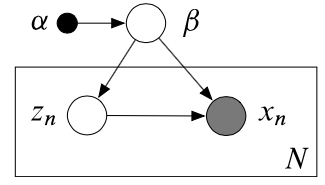
\includegraphics[width=0.35\textwidth]{LVM.png}
  \end{center}
  \end{figure}

  Models with
  \begin{itemize}
  \item Small(ish) set of \emph{global} parameters: $\beta$
  \item Large set of \emph{latent variables} or \emph{local} parameters: $z$
  \end{itemize}

  Examples:
  \begin{itemize}
  \item Gaussian mixture model: Global parameters are the means,
    variances and prior weights, local parameters are the sample
    allocations
  \item Topic model: Global parameters are topic-to-word distributions,
    local parameters are the document-to-topic distributions
  \end{itemize}
\end{frame}

\begin{frame}
  \frametitle{Variational inference basics}

  \begin{itemize}
  \item Idea: approximate the posterior distribution $p(\beta, z| \dataset)$
    with another distribution $q(\beta,z|\lambda,\phi)$ that is more
    tractable
  \item Learn the approximation by minimizing the distance between $q(\beta,z|\lambda,\phi)$ and $p(\beta, z |\dataset)$
  \item The distance is measured by the Kullback-Leibler divergence
    $D(q||p) = \int q(\beta,z) \log \frac{q(\beta,z)}{p(\beta,z| \dataset)}\diff \beta \diff z$
  \item ...and the minimization is often converted into maximizing a lower bound on the marginal
    likelihood (ELBO):
    $L = \int q(\beta,z) \log \frac{p(\dataset,\beta,z)}{q(\beta,z)} \diff \beta \diff z = p(\dataset) - D(q||p)$
  \item Predictions made by integrating over the approximation
  \end{itemize}

  Converts Bayesian inference into an optimization problem!
\end{frame}

\begin{frame}
  \frametitle{Variational inference basics}

  \begin{figure}
  \begin{center}
  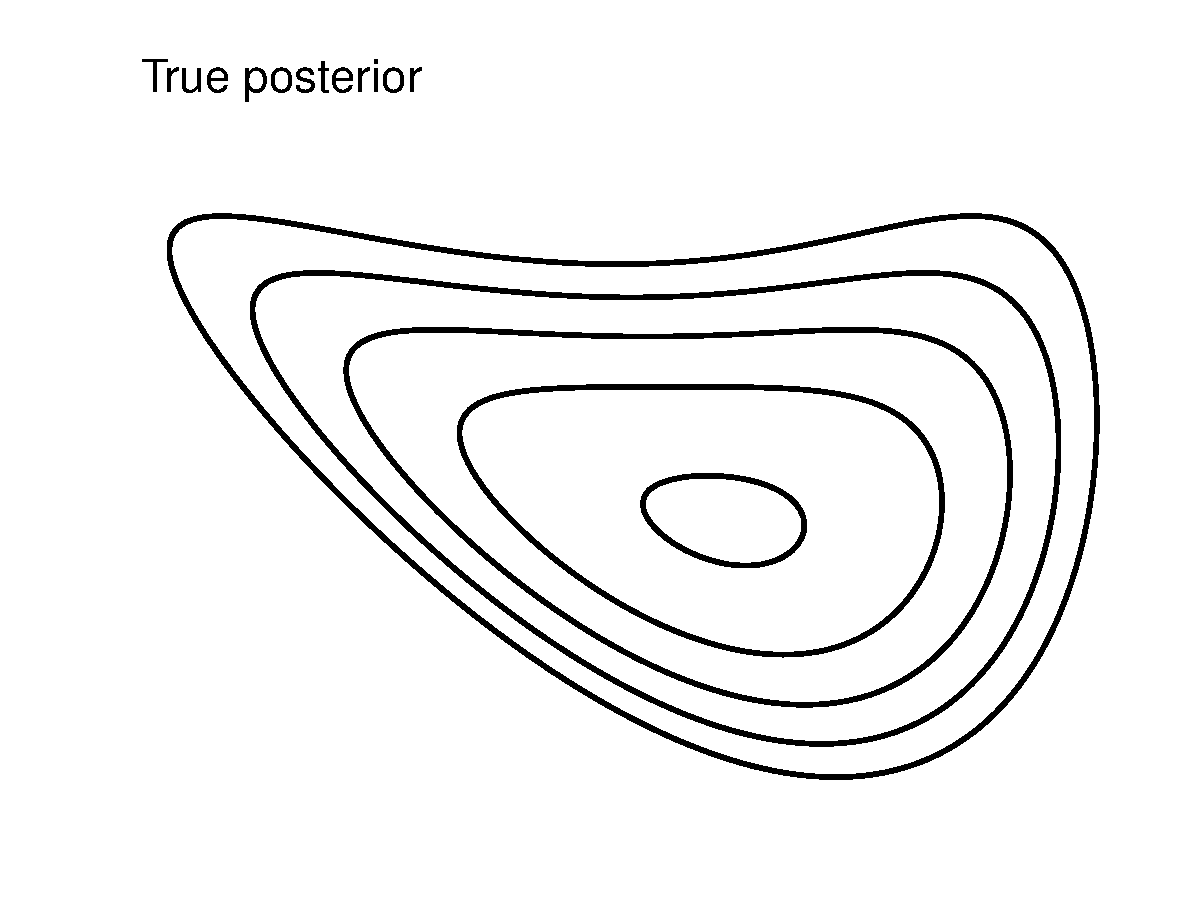
\includegraphics[width=0.7\textwidth]{VBexample1.pdf}
  \end{center}
  \end{figure}

\end{frame}

\begin{frame}
  \frametitle{Variational inference basics}

  \begin{figure}
  \begin{center}
  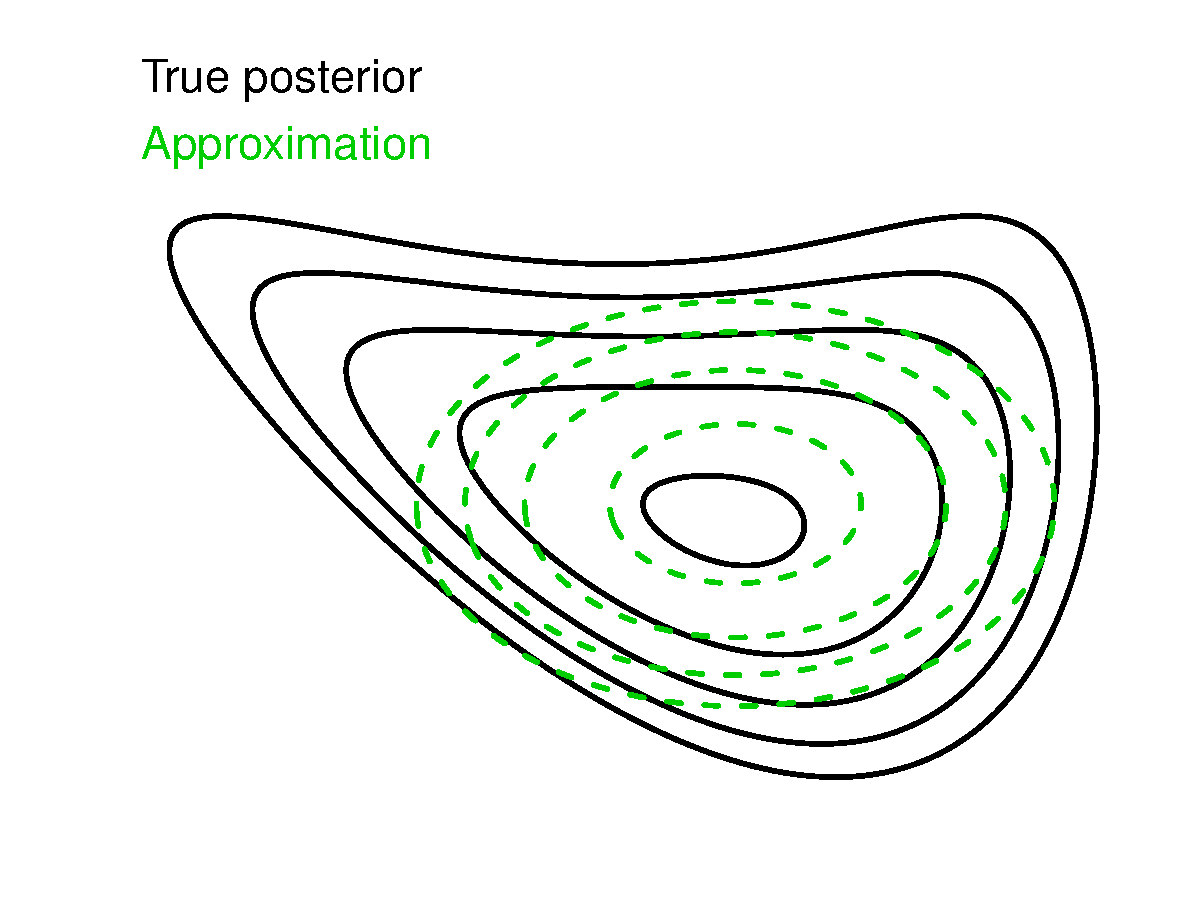
\includegraphics[width=0.7\textwidth]{VBexample2.pdf}
  \end{center}
  \end{figure}

\end{frame}

\begin{frame}
  \frametitle{Mean-field variational inference}

  Latent variable model:\\
  Global parameter $\beta$, global variational parameter $\lambda$\\
  Local parameters $z_i$, local variational parameters $\phi_i$

  \begin{itemize}
    \item Mean-field approximation:
      $q(\beta,z) = q(\beta|\lambda) \prod_{i}^n q(z_i|\phi_i)$
    \item As a function of $\lambda$, the cost function becomes
      $L(\lambda) = \langle \log p(\beta|\dataset,z)
      - \log q(\beta|\lambda)\rangle_{q} + \text{const}$
    \item Gradient-based optimization directly applicable, for each
      term at a time
  \end{itemize}
\end{frame}

\begin{frame}
  \frametitle{Gradients and exponential families}

  Exponential family:
  \begin{align*}
  p(\beta|\dataset,z) &= h_p(\beta) e^{\eta^T t(\beta) - a_p(\eta)} \\
  q(\beta|\lambda) &= h_q(\beta) e^{\lambda^T t(\beta) - a_q(\lambda)}
  %\langle \log p(\beta|\dataset,z) \rangle &= \langle \eta \rangle^T \nabla a_q(\lambda) + \text{const}\\
  %\langle \log q(\beta|\lambda) \rangle &= \lambda^T \nabla a_q(\lambda) - a_q(\lambda)
  \end{align*}
  ...with nice property $\langle t(\beta) \rangle_q = \nabla a_q(\lambda)$

  \begin{itemize}
    \item The cost function becomes
      $L(\lambda) = \langle \eta \rangle^T_q \nabla a_q(\lambda)
      - \lambda^T \nabla a_q(\lambda) + a_q(\lambda) + \text{const}$
    \item ...and the gradient hence
      $\nabla L(\lambda) = \nabla^2 a_q(\lambda)
      (\langle \eta \rangle_q - \lambda)$
    \item Closed-form updates $\lambda = \langle \eta \rangle_q$
      where $\eta$ is some function of the data and the local
      parameters
  \end{itemize}
  Note the close relationship with Gibbs sampling: Now we take the
  expectation of the conditional instead of sampling from it!
\end{frame}

\begin{frame}
  \frametitle{Mean-field variational inference}

  \begin{itemize}
    \item The Bayesian inference now converted into an optimization
      problem with simple EM-like alternating updates
    \item Computation similar to Gibbs samplers, but often converges
      in tens/hundreds of iterations
    \item Complexity still $\mathcal{O}(n)$, since evaluating the
      expectation $\langle \eta \rangle_q$ requires processing all data points
  \end{itemize}
\end{frame}

\begin{frame}
  \frametitle{Gradient descent and natural gradients}

  \begin{itemize}
    \item Gradient descent: $\lambda^t \leftarrow \lambda^{t-1}
      + \rho_t \nabla L(\lambda)$
    \item Natural gradients: Pre-multiply with the inverse Fisher
      information matrix for faster convergence
    \item In the exponential family makes things simpler since
      the term $\nabla^2 a(\vparameters_i)$ disappears:
      $\nabla L(\lambda) = \langle \eta \rangle_q - \lambda$
  \end{itemize}
  \begin{figure}
  \begin{center}
  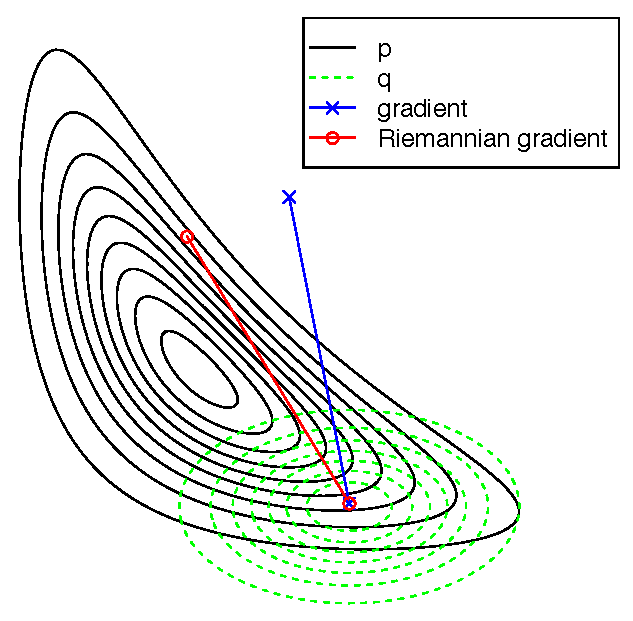
\includegraphics[width=0.4\textwidth]{VBnatgrad.pdf}
  \end{center}
  \end{figure}
  \vfill \hfill {\tiny Figure from Honkela et al. (JMLR 2010)}
\end{frame}

\begin{frame}
  \frametitle{Stochastic gradients}

  \begin{itemize}
    \item Computing the gradient still takes $\mathcal{O}(n)$
    \item Stochastic optimization to the rescue:
      Instead of evaluating the gradient exactly, we can use
      an (unbiased) estimate
    \item Basic idea: Replace the natural gradient
      $\nabla L(\lambda) = \langle \eta \rangle_q - \lambda$
      with stochastic estimate based on one (or a few) data point
    \item Robbins-Monro (1951): Stochastic gradient descent
      finds the correct optimum if step lengths $\rho_t$ decrease
      over time so that $\sum_t \rho_t = \infty$ and $\sum_t \rho_t^2 < \infty$
  \end{itemize}
\end{frame}

\begin{frame}
  \frametitle{Stochastic variational inference}

  The above ideas properly formulated by
  M.D. Hoffman, D.M. Blei, C. Wang, and J. Paisley. \textbf{Stochastic Variational Inference}, JMLR 2013

  \begin{figure}
  \begin{center}
  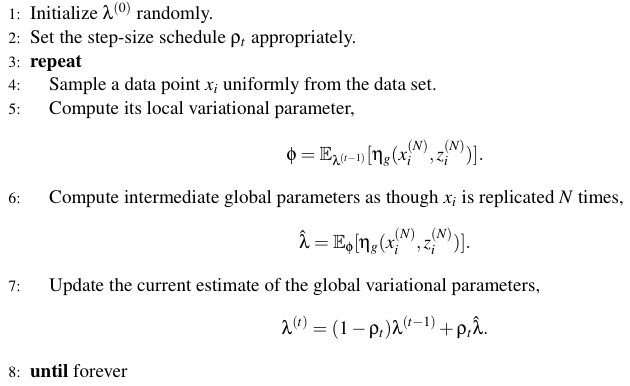
\includegraphics[width=0.7\textwidth]{SVI.png}
  \end{center}
  \end{figure}

\end{frame}

\begin{frame}
  \frametitle{Stochastic variational inference}

  \begin{figure}
  \begin{center}
  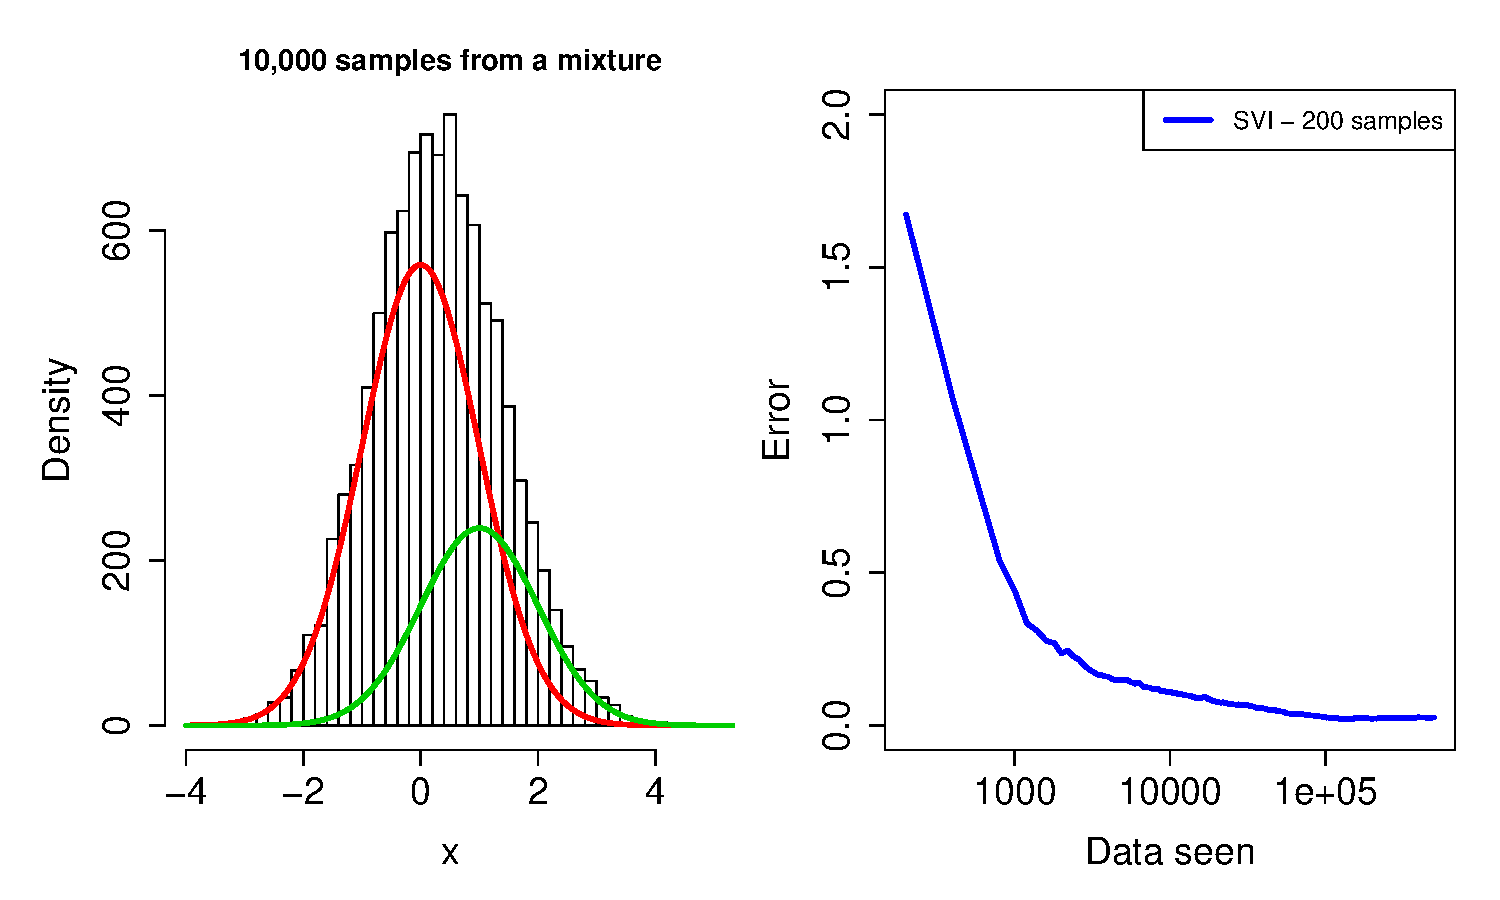
\includegraphics[width=0.9\textwidth]{mixture1.pdf}
  \end{center}
  \end{figure}

\end{frame}

\begin{frame}
  \frametitle{Stochastic variational inference}

  \begin{figure}
  \begin{center}
  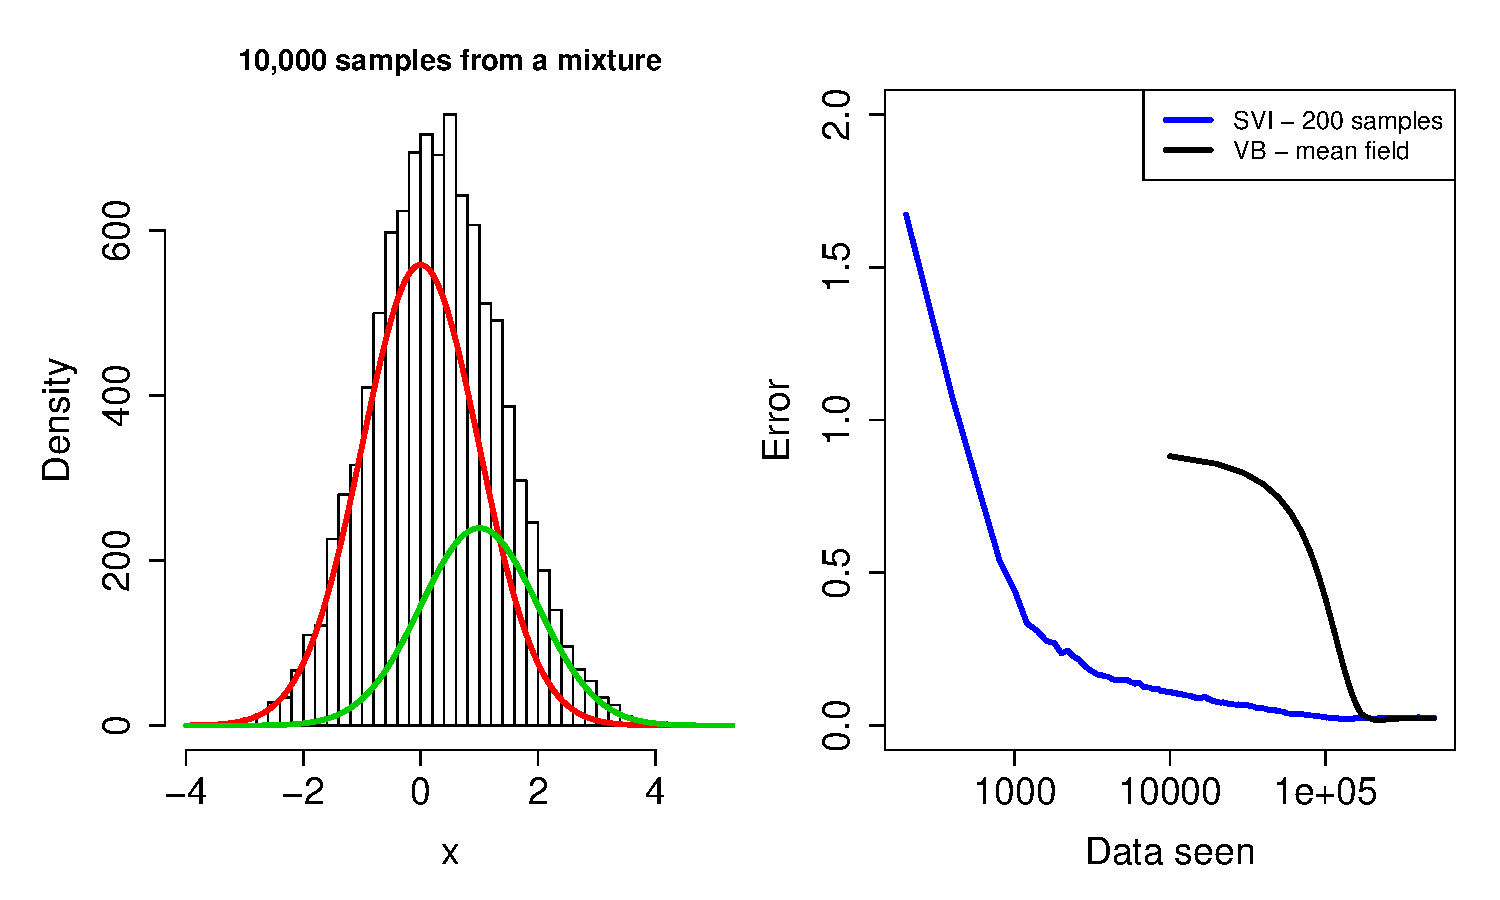
\includegraphics[width=0.9\textwidth]{mixture2.pdf}
  \end{center}
  \end{figure}

\end{frame}

\begin{frame}
  \frametitle{Stochastic variational inference}

  \begin{figure}
  \begin{center}
  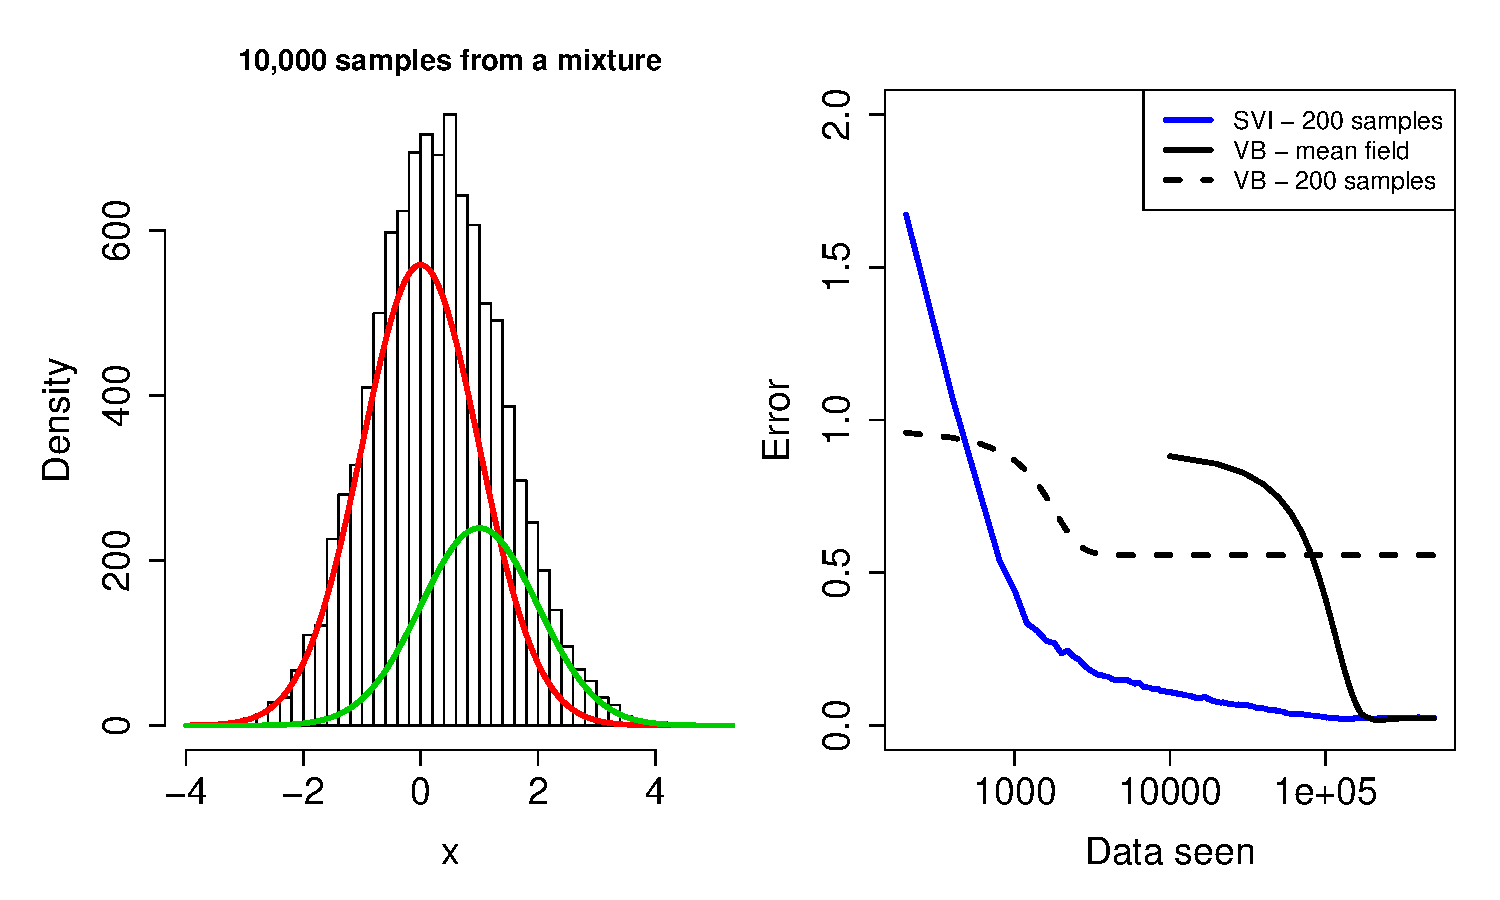
\includegraphics[width=0.9\textwidth]{mixture3.pdf}
  \end{center}
  \end{figure}

\end{frame}

\begin{frame}
  \frametitle{Stochastic variational inference in practice}

  \begin{itemize}
  \item Stochastic optimization has theoretical guarantees, but
    practical convergence depends heavily on the details
  \item Several ways of adapting step lengths etc presented over
    the years in the optimization community, resulting in various
    theoretical convergence rates
  \item Some practical tools: Adagrad, Nesterov's method, Smoothing
  \item Active research topic: ML community currently pushing out
    a lot of papers on both improving the convergence and/or speed,
    and on presenting the algorithmic details for slightly more general setups
  \end{itemize}
\end{frame}



%\begin{frame}
%  \frametitle{Some more elaborate examples}

%  \begin{enumerate}
%  \item J. Hensman, N. Fusi, N.D. Lawrence, \textbf{Gaussian Processes for Big Data}, UAI 2013.
%  \item J. M. Hernandez-Lobato, N. Houlsby, Z. Ghahramani, \textbf{Stochastic Inference for Scalable Probabilistic Modeling of Binary Matrices}, ICML 2014.
%  \end{enumerate}

%  \begin{itemize}
%  \item GP inference
%    $$ y_i = f(\vx_i) + \epsilon $$
%  \item Variational sparse GPs: introduce \emph{inducing variables}
%    $$ \mathbf{u} = [f(\mathbf{z}_i)]_{i=1}^m $$
%  \item Standard variational GPs collapse $\mathbf{u}$, but that
%    cannot be done with SVI
%  \end{itemize}

%  \begin{itemize}
%  \item Subsample both data points and ``global variables''
%  \item Nice method for deciding mini-batch size
%  \end{itemize}
%\end{frame}

%\section{Other}

%\begin{frame}
  % Arto + Antti
%  \frametitle{Stochastic gradients in general}

%  \begin{enumerate}
%  \item M. Schmidt, N. Le Roux, F. Bach, \textbf{Minimizing Finite Sums with the Stochastic Average Gradient}, arXiv 2013.
%  \end{enumerate}
%  \begin{itemize}
%  \item Basic idea: introduce a memory of gradients and simply update the
%    component from one data point or mini-batch at a time
%  \item Improves the asymptotic convergence rate
%  \end{itemize}

%\end{frame}


\section{MCMC}

% Antti

\begin{frame}
  % Antti
  \frametitle{Approximate inference by sampling}

  \begin{itemize}
  \item A lot of Bayesian inference boils down to computing integrals
    $$ E[f(\parameters)] = \int_\parameters f(\parameters) p(\parameters | \dataset) \diff\parameters $$
    \begin{itemize}
    \item Model predictions, posterior statistics of parameters, \dots
    \end{itemize}
  \item $\parameters$ is often high-dimensional which makes these very difficult
  \item Stochastic approximation:
    $$ E[f(\parameters)] \approx \frac{1}{N} \sum_{i=1}^N f(\parameters_i), $$
    when $\parameters_i \sim p(\parameters | \dataset)$
  \item How to simulate samples following a given distribution?
  \end{itemize}
\end{frame}

\begin{frame}
  \frametitle{MCMC basics (Metropolis et al., 1953; Hastings, 1970)}

  \begin{itemize}
  \item Idea: construct a Markov chain, whose stationary distribution
    is the distribution of interest $p(\parameters | \dataset)$
  \item Requires an \emph{unnormalised} $p^*(\parameters | \dataset) \propto
    p(\parameters | \dataset)$
  \item In the Bayesian setting typically
    $$ p(\parameters | \dataset) = \frac{p(\dataset | \parameters) p(\parameters)}{p(\dataset)} $$
    which easily yields the unnormalised density
    $$ p^*(\parameters | \dataset) = p(\dataset | \parameters) p(\parameters) $$
  \item To define the Markov chain, we need to specify a transition
    distribution $q(\parameters' | \parameters)$
  \item The Markov chain is guaranteed to converge if it satisfies
    sufficient regularity conditions and the \emph{detailed balance}
    condition
    $$ q(\parameters' | \parameters) p(\parameters | \dataset) =
       q(\parameters | \parameters') p(\parameters' | \dataset) $$
  \end{itemize}
\end{frame}

\begin{frame}
  \frametitle{Metropolis--Hastings algorithm}

  \begin{itemize}
  \item The most widely used MCMC algorithm is the Metropolis--Hastings
    algorithm
  \item Accept--reject mechanism, proposals are accepted with probability
    $$ f(\parameters' | \parameters) = \min\left(1, \frac{\color{blue}q(\parameters | \parameters') p(\parameters' | \dataset)}
      {\color{red}q(\parameters' | \parameters) p(\parameters | \dataset)} \right) $$
  \item This satisfies the detailed balance because
    \begin{align*}
      {\color{red}f(\parameters' | \parameters)
      q(\parameters' | \parameters) p(\parameters | \dataset)}
      &= \min({\color{blue}q(\parameters' | \parameters) p(\parameters | \dataset)},
      {\color{red}q(\parameters | \parameters') p(\parameters' | \dataset)}) \\
      &= \min({\color{red}q(\parameters | \parameters') p(\parameters' | \dataset)},
      {\color{blue}q(\parameters' | \parameters) p(\parameters | \dataset)}) \\
      &= {\color{blue}f(\parameters | \parameters')
      q(\parameters | \parameters') p(\parameters' | \dataset)}
    \end{align*}
  \end{itemize}
\end{frame}

\begin{frame}
  \frametitle{MCMC for big data}

  \begin{itemize}
  \item The challenge for big data: likelihood computation needed for
    acceptance decision needs all data
  \item Proposed solutions
    \begin{enumerate}
    \item Work on subsets of data
    \item Approximate the acceptance decision
    \item Make better proposals that avoid acceptance checks
    \end{enumerate}
  \end{itemize}
\end{frame}

\begin{frame}
  \frametitle{Solution 1: Subset and parallelised sampling}

  \begin{enumerate}
  \item D. Maclaurin, R.P. Adams, \textbf{Firefly Monte Carlo: Exact MCMC with Subsets of Data}, UAI 2014.
  \item W. Neiswanger, E. Xing, C. Wang, \textbf{Asymptotically Exact, Embarrassingly Parallel MCMC}, UAI 2014; S.L. Scott, A.W. Blocker, F.V. Bonassi, H.A. Chipman, E.I. George, R.E. McCulloch, \textbf{Bayes and Big Data: The Consensus Monte Carlo Algorithm}, Bayes 250, 2013; and T. Campbell, J. How, \textbf{Approximate Decentralized Bayesian Inference}, UAI 2014. 
  \end{enumerate}
\end{frame}

\begin{frame}
  \frametitle{Solution 2: Approximate acceptance}

  \begin{enumerate}
  \item A. Korattikara, Y. Chen, M. Welling, \textbf{Austerity in MCMC Land: Cutting the Metropolis--Hastings Budget}, ICML 2014.
  \end{enumerate}

  \begin{itemize}
  \item Basic idea: more efficient use of data by approximating the
    Metropolis--Hastings accept/reject choice
  \end{itemize}
\end{frame}

\begin{frame}
  % Antti
  \frametitle{Solution 3: Better proposals using gradients}
  % HMC etc

  \begin{itemize}
  \item Standard MCMC is based on proposal distributions whose shape is
    essentially \emph{independent of the target}
    \begin{itemize}
    \item E.g.~fixed multivariate Gaussian proposals
    \end{itemize}
  \item Target distribution gradients would allow utilising local shape
  \item Common algorithms:
    \begin{itemize}
    \item Langevin dynamics MCMC
    \item Hamiltonian Monte Carlo  (a.k.a. hybrid Monte Carlo)
    \end{itemize}
  \item Both based on constructing a suitable dynamical system and
    simulating it
  \end{itemize}
\end{frame}

\begin{frame}
  \frametitle{Langevin and Hamiltonian dynamics in MCMC}

  Langevin dynamics proposal:
  $$ \parameters^* = \parameters + \frac{\epsilon}{2} \nabla_\parameters p(\dataset, \parameters) + N(0, \epsilon I) $$
  \begin{itemize}
  \item Acceptance rate tends to one as $\epsilon \rightarrow 0$
  \end{itemize}
  \mbox{}\\
  Hamiltonian MCMC:
  \begin{itemize}
  \item Construct a Hamiltonian dynamical system with momentum
  \item Hamiltonian ($\approx$ ``energy'') is conserved in simulation
  \item Can take arbitrarily long steps, assuming the Hamiltonian
    system can be simulated accurately
    \begin{itemize}
    \item Symplectic geometry studies this problem
    \end{itemize}
  \end{itemize}
\end{frame}

\begin{frame}[allowframebreaks]
  % Arto + Antti
  \frametitle{Stochastic gradients with MCMC}

  \begin{enumerate}
  \item M. Welling, Y.W.Teh, \textbf{Bayesian Learning via Stochastic Gradient Langevin Dynamics}, ICML 2011 and S. Ahn, A. Korattikara, M. Welling, \textbf{Bayesian posterior sampling via stochastic gradient Fisher scoring}, ICML 2012.
  \item T. Chen, E. Fox, C. Guestrin, \textbf{Stochastic Gradient Hamiltonian Monte Carlo}, ICML 2014.
  \end{enumerate}

  \begin{itemize}
  \item Stochastic gradient proposal, always accept
  \item Convergence needs step sizes shrinking to zero, not usually done
  \end{itemize}
\end{frame}


\begin{frame}
  \frametitle{Summary}

  \begin{itemize}
  \item VB algorithms rest on solid theoretical foundation with SGD
  \item Ensuring convergence in practice can still be tricky
  \item Big data MCMC theoretical analysis still developing
  \item Cautionary tales from skipping MH-step
  \item Subset and austerity approaches seem more reliable, but may
    still have gotchas
  \end{itemize}
\end{frame}


\end{document}
